\chapter{函数}

\section{函数}

\subsection{函数(Function)}

函数执行一个特定的任务,Python提供了大量内置函数,例如print()用来输出字符串、len()用来计算序列长度等。

\begin{figure}[H]
	\centering
	\begin{tikzpicture}[scale=0.5]
		\draw[-] (5,-2) -- (10,-2) -- (10,2) -- (5,2) -- (5,-2);
		\draw[->] (0,0) -- (5,0);
		\draw[->] (10,0) -- (15,0);

		\draw (-2,0) node {Input};
		\draw (17,0) node {Output};
		\draw (7.5,0) node {Function};
	\end{tikzpicture}
	\caption{函数}
\end{figure}

当调用函数时,程序控制权会转移给被调用的函数,当函数执行结束后,函数会把程序序控制权交还给其调用者。

\begin{figure}[H]
	\centering
	\begin{tikzpicture}[]
		\draw (0,4.5) node {Caller};
		\draw[->] (0,4) -- (0,0.5);
		\draw[->] (0,-0.5) -- (0,-4);
		\draw (0,0) node {调用foo()};

		\draw (4,4) node {foo()};
		\draw[->] (4,3) -- (4,0.5);
		\draw[->] (4,-0.5) -- (4,-3);
		\draw (4,0) node {调用bar()};

		\draw (8,3) node {bar()};
		\draw[->] (8,2) -- (8,-2);

		\draw[->] (0.5,0.5) -- (3.5,3);
		\draw[->] (3.5,-3) -- (0.5,-0.5);
		\draw[->] (4.5,0.5) -- (7.5,2);
		\draw[->] (7.5,-2) -- (4.5,-0.5);
	\end{tikzpicture}
	\caption{函数调用}
\end{figure}

使用def关键字可以定义函数:

\begin{lstlisting}[language=Python]
def func_name([param_list]):
    # code
\end{lstlisting}

\vspace{0.5cm}

\subsection{函数设计方法}

为什么不把所有的代码全部写在一起,还需要自定义函数呢?\\

使用函数有以下好处:

\begin{enumerate}
	\item 避免代码复制,代码复制是程序质量不良的表现
	\item 便于代码维护
	\item 避免重复造轮子,提高开发效率
\end{enumerate}

在设计函数的时候需要考虑以下的几点要素:

\begin{enumerate}
	\item 确定函数的功能

	\item 确定函数的参数
	      \begin{itemize}
		      \item 是否需要参数
		      \item 参数个数
		      \item 参数类型
	      \end{itemize}

	\item 确定函数的返回值
	      \begin{itemize}
		      \item 是否需要返回值
		      \item 返回值类型
	      \end{itemize}
\end{enumerate}

\mybox{函数实现返回最大值}

\begin{lstlisting}[language=Python]
def get_max(num1, num2):
    # if num1 > num2:
    #     return num1
    # else:
    #     return num2

    return num1 if num1 > num2 else num2

print(get_max(4, 12))
print(get_max(54, 33))
print(get_max(0, -12))
print(get_max(-999, -774))
\end{lstlisting}

\begin{tcolorbox}
	\mybox{运行结果}
	\begin{verbatim}
12
54
0
-774
\end{verbatim}
\end{tcolorbox}

\vspace{0.5cm}

\mybox{函数实现累加和}

\begin{lstlisting}[language=Python]
def get_sum(start, end):
    total = 0
    for i in range(start, end+1):
        total += i
    return total

print("1-100的累加和 = %d" % get_sum(1, 100))
print("1024-2048的累加和 = %d" % get_sum(1024, 2048))
\end{lstlisting}

\begin{tcolorbox}
	\mybox{运行结果}
	\begin{verbatim}
1-100的累加和 = 5050
1024-2048的累加和 = 1574400
\end{verbatim}
\end{tcolorbox}

\vspace{0.5cm}

\mybox{函数实现输出i行j列由自定义字符组成的图案}

\begin{lstlisting}[language=Python]
def print_chars(row, col, c):
    for i in range(row):
        for j in range(col):
            print(c, end='')
        print()

print_chars(5, 10, '?')
\end{lstlisting}

\begin{tcolorbox}
	\mybox{运行结果}
	\begin{verbatim}
??????????
??????????
??????????
??????????
??????????
\end{verbatim}
\end{tcolorbox}

\newpage

\section{主函数}

\subsection{主函数}

Python是为数不多的直接定义完源代码就可以执行的编程语言,很多编程语言对于程序的执行都有非常严格的标准,例如C、C++、Java等都有主函数(主方法)来标记程序的起点。\\

在现实的开发之中主函数是很有必要的,可以区分出其它的结构,在模块中更需要主函数的使用。\\

在Python中如果想实现主函数的定义,必须借助于全局变量\_\_name\_\_的返回内容,而后采用自定义的函数形式实现,返回的\_\_main\_\_是一个字符串,这个内容是会改变的,跟程序身处的结构有关。\\

在很多的编程语言都将主函数通过main这个标识符来定义,所以定义的main()是符合一般的习惯的。在进行复杂开发的时候,强烈建议使用主函数作为程序的起点。\\

\mybox{主函数}

\begin{lstlisting}[language=Python]
def main():
    pass

if __name__ == "__main__":
    main()
\end{lstlisting}

\newpage

% \section{递归} \label{recursive}

% \subsection{递归(Recursion)}

% 要理解递归,先得理解递归(见\ref{recursive}章节)。\\

% 在函数的内部,直接或者间接的调用自己的过程就叫作递归。对于一些问题,使用递归可以简洁易懂的解决问题,但是递归的缺点是性能低,占用大量系统栈空间。\\

% 递归算法很多时候可以处理一些特别复杂、难以直接解决的问题。例如:

% \begin{itemize}
% 	\item 迷宫
% 	\item 汉诺塔
% 	\item 八皇后
% 	\item 排序
% 	\item 搜索
% \end{itemize}

% 在定义递归函数时,一定要确定一个结束条件,否则会造成无限递归的情况,最终会导致栈溢出。

% \begin{figure}[H]
% 	\centering
% 	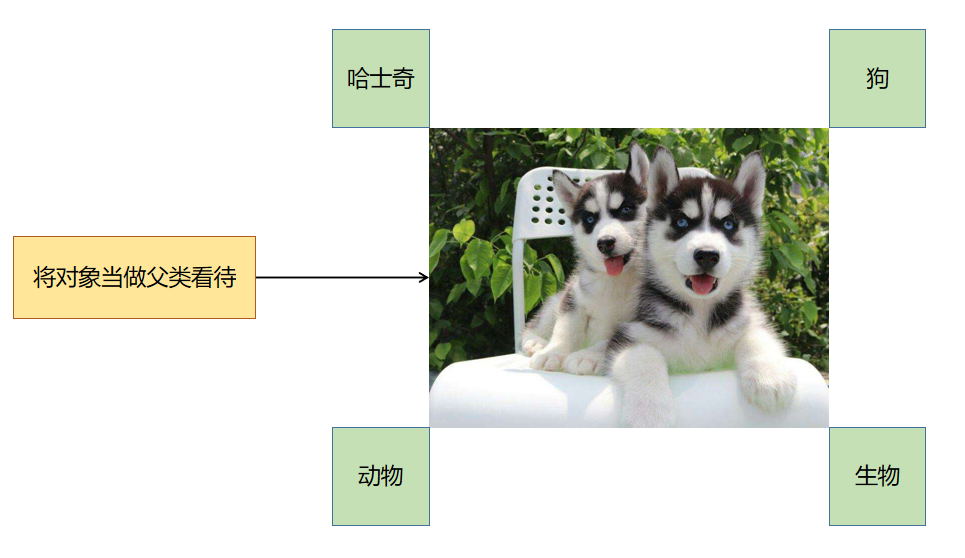
\includegraphics[scale=0.7]{img/C6/6-2/1.png}
% \end{figure}

% \begin{figure}[H]
% 	\centering
% 	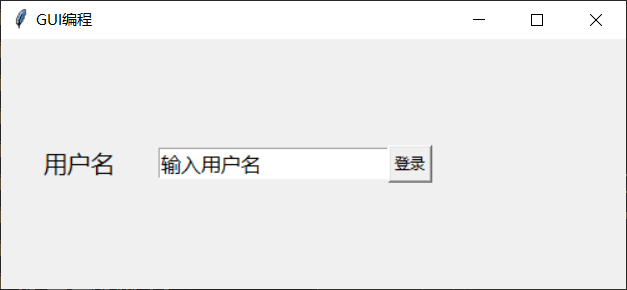
\includegraphics[scale=0.6]{img/C6/6-2/2.png}
% \end{figure}

% \begin{figure}[H]
% 	\centering
% 	
\includegraphics[scale=0.6]{img/C6/6-2/3.png}
% \end{figure}

% \begin{figure}[H]
% 	\centering
% 	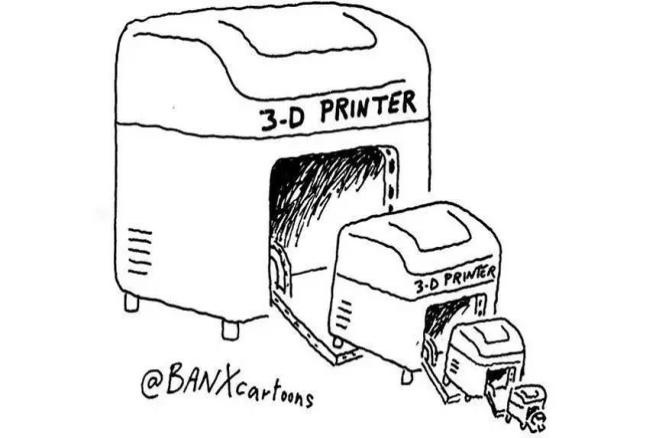
\includegraphics[scale=1.3]{img/C6/6-2/4.png}
% \end{figure}

% \begin{figure}[H]
% 	\centering
% 	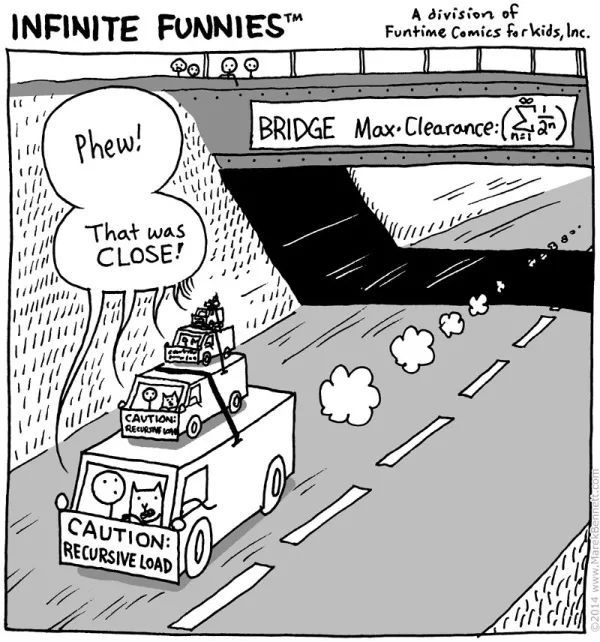
\includegraphics[scale=0.6]{img/C6/6-2/5.png}
% \end{figure}

% \mybox{无限递归}

% \begin{lstlisting}[language=Python]
% public class TellStory {
% 	public static void main(String[] args) {
% 		tellStory();
% 	}

% 	public static void tellStory() {
% 		System.out.println("从前有座山");
% 		System.out.println("山里有座庙");
% 		System.out.println("庙里有个老和尚和小和尚");
% 		System.out.println("老和尚在对小和尚讲故");
% 		System.out.println("他讲的故事是:");
% 		tellStory();
% 	}
% }
% \end{lstlisting}

% \begin{tcolorbox}
% 	\mybox{运行结果}
% 	\begin{verbatim}
% 从前有座山
% 山里有座庙
% 庙里有个老和尚和小和尚
% 老和尚对小和尚在讲故事
% 他讲的故事是:
% 从前有座山
% 山里有座庙
% 庙里有个老和尚和小和尚
% 老和尚对小和尚在讲故事
% 他讲的故事是:
% ...
% \end{verbatim}
% \end{tcolorbox}

% 递归函数一般需要定义递归的出口,即结束条件,确保递归能够在适合的地方退出。\\

% \mybox{阶乘}

% \begin{lstlisting}[language=Python]
% public class Factorial {
% 	public static void main(String[] args) {
% 		System.out.println("5! = " + factorial(5));
% 	}

% 	public static int factorial(int n) {
% 		if(n == 0 || n == 1) {
% 			return 1;
% 		}
% 		return n * factorial(n-1);
% 	}
% }
% \end{lstlisting}

% \begin{tcolorbox}
% 	\mybox{运行结果}
% 	\begin{verbatim}
% 5! = 120
% \end{verbatim}
% \end{tcolorbox}

% \begin{figure}[H]
% 	\centering
% 	\begin{tikzpicture}[]
% 		\draw (0,0) rectangle (3,1.5);
% 		\draw (3,-2) rectangle (6,-0.5);
% 		\draw (6,-4) rectangle (9,-2.5);
% 		\draw (9,-6) rectangle (12,-4.5);
% 		\draw (12,-8) rectangle (15,-6.5);

% 		\draw (12.75,-10.75) rectangle (14.25,-9.25);
% 		\draw (9.75,-8.75) rectangle (11.25,-7.25);
% 		\draw (6.75,-6.75) rectangle (8.25,-5.25);
% 		\draw (3.75,-4.75) rectangle (5.25,-3.25);
% 		\draw (0.75,-2.75) rectangle (2.25,-1.25);

% 		\draw (1.5,0.75) node {$ factorial(5) $};
% 		\draw (4.5,-1.25) node {$ factorial(4) $};
% 		\draw (7.5,-3.25) node {$ factorial(3) $};
% 		\draw (10.5,-5.25) node {$ factorial(2) $};
% 		\draw (13.5,-7.25) node {$ factorial(1) $};

% 		\draw (13.5,-10) node {$ 1 $};
% 		\draw (10.5,-8) node {$ 2 $};
% 		\draw (7.5,-6) node {$ 6 $};
% 		\draw (4.5,-4) node {$ 24 $};
% 		\draw (1.5,-2) node {$ 120 $};

% 		\draw[->] (3,0.75) -- (4.5,0.75) -- (4.5,-0.5);
% 		\draw[->] (6,-1.25) -- (7.5,-1.25) -- (7.5,-2.5);
% 		\draw[->] (9,-3.25) -- (10.5,-3.25) -- (10.5,-4.5);
% 		\draw[->] (12,-5.25) -- (13.5,-5.25) -- (13.5,-6.5);

% 		\draw[->] (12.75,-10) -- (10.5,-10) -- (10.5,-8.75);
% 		\draw[->] (9.75,-8) -- (7.5,-8) -- (7.5,-6.75);
% 		\draw[->] (6.75,-6) -- (4.5,-6) -- (4.5,-4.75);
% 		\draw[->] (3.75,-4) -- (1.5,-4) -- (1.5,-2.75);

% 		\draw (4.5,1) node {$ 5 * factorial(4) $};
% 		\draw (7.5,-1) node {$ 4 * factorial(3) $};
% 		\draw (10.5,-3) node {$ 3 * factorial(2) $};
% 		\draw (13.5,-5) node {$ 2 * factorial(1) $};

% 		\draw (11,-10.5) node {$ 2 * 1 $};
% 		\draw (8,-8.5) node {$ 3 * 2 $};
% 		\draw (5,-6.5) node {$ 4 * 6 $};
% 		\draw (2,-4.5) node {$ 5 * 24 $};
% 	\end{tikzpicture}
% 	\caption{阶乘}
% \end{figure}

% \mybox{斐波那契数列(递归)}

% \begin{lstlisting}[language=Python]
% public class FibonacciRecursive {
% 	public static void main(String[] args) {
% 		int n = 7;
% 		System.out.println(
% 			"斐波那契数列第" + n + "位:"+ fibonacci(n)
% 		);
% 	}

% 	public static int fibonacci(int n) {
% 		if(n == 1 || n == 2) {
% 			return 1;
% 		}
% 		return fibonacci(n-2) + fibonacci(n-1);
% 	}
% }
% \end{lstlisting}

% \begin{tcolorbox}
% 	\mybox{运行结果}
% 	\begin{verbatim}
% 斐波那契数列第7位:13
% \end{verbatim}
% \end{tcolorbox}

% \begin{figure}[H]
% 	\centering
% 	\begin{tikzpicture}[
% 			level distance=2.4cm,
% 			level 1/.style={sibling distance=6cm},
% 			level 2/.style={sibling distance=3cm},
% 			level 3/.style={sibling distance=2cm}
% 		]
% 		\node {$ f(5) $}
% 		child {
% 				node {$ f(3) $}
% 				child {node {$ f(1) $}}
% 				child {
% 						node {$ f(2) $}
% 						child {node {$ f(0) $}}
% 						child {node {$ f(1) $}}
% 					}
% 			}
% 		child {
% 				node {$ f(4) $}
% 				child {
% 						node {$ f(2) $}
% 						child {node {$ f(0) $}}
% 						child {node {$ f(1) $}}
% 					}
% 				child {
% 						node {$ f(3) $}
% 						child {node {$ f(1) $}}
% 						child {
% 								node {$ f(2) $}
% 								child {node {$ f(0) $}}
% 								child {node {$ f(1) $}}
% 							}
% 					}
% 			};
% 	\end{tikzpicture}
% 	\caption{递归树}
% \end{figure}

% \mybox{斐波那契数列(迭代)}

% \begin{lstlisting}[language=Python]
% public class FibonacciIterative {
% 	public static void main(String[] args) {
% 		int n = 7;
% 		System.out.println(
% 			"斐波那契数列第" + n + "位:"+ fibonacci(n)
% 		);
% 	}

% 	public static int fibonacci(int n) {
% 		int[] f = new int[n];
% 		f[0] = f[1] = 1;
% 		for(int i = 2; i < n; i++) {
% 			f[i] = f[i-2] + f[i-1];
% 		}
% 		return f[n-1];
% 	}
% }
% \end{lstlisting}

% \begin{tcolorbox}
% 	\mybox{运行结果}
% 	\begin{verbatim}
% 斐波那契数列第7位:13
% \end{verbatim}
% \end{tcolorbox}

% \vspace{0.5cm}

% \mybox{阿克曼函数}

% \begin{align}\nonumber
% 	A(m, n) =
% 	\begin{cases}
% 		n + 1             & m = 0        \\
% 		A(m-1, 1)         & m > 0, n = 0 \\
% 		A(m-1, A(m, n-1)) & m > 0, n > 0 \\
% 	\end{cases}
% \end{align}

% \begin{lstlisting}[language=Python]
% public class Ackermann {
% 	public static void main(String[] args) {
% 		System.out.println(A(3, 4));
% 	}

% 	public static int A(int m, int n) {
% 		if(m == 0) {
% 			return n + 1;
% 		} else if(m > 0 && n == 0) {
% 			return A(m-1, 1);
% 		} else {
% 			return A(m-1, A(m, n-1));
% 		}
% 	}
% }
% \end{lstlisting}

% \begin{tcolorbox}
% 	\mybox{运行结果}
% 	\begin{verbatim}
% 125
% \end{verbatim}
% \end{tcolorbox}

% \begin{table}[H]
% 	\centering
% 	\setlength{\tabcolsep}{0.5mm}{
% 		\begin{tabular}{|c|c|c|c|c|c|c|}
% 			\hline
% 			\diagbox{$ m $}{$ n $} & \textbf{$ 0 $} & \textbf{$ 1 $}    & \textbf{$ 2 $}    & \textbf{$ 3 $}          & \textbf{$ 4 $}    & \textbf{$ n $}                                         \\
% 			\hline
% 			\textbf{$ 0 $}         & $ 1 $          & $ 2 $             & $ 3 $             & $ 4 $                   & $ 5 $             & $ n + 1 $                                              \\
% 			\hline
% 			\textbf{$ 1 $}         & $ 2 $          & $ 3 $             & $ 4 $             & $ 5 $                   & $ 6 $             & $ 2 + (n + 3) - 3 $                                    \\
% 			\hline
% 			\textbf{$ 2 $}         & $ 3 $          & $ 5 $             & $ 7 $             & $ 9 $                   & $ 11 $            & $ 2(n + 3) - 3 $                                       \\
% 			\hline
% 			\textbf{$ 3 $}         & $ 5 $          & $ 13 $            & $ 29 $            & $ 61 $                  & $ 125 $           & $ 2^{n + 3} - 3 $                                      \\
% 			\hline
% 			\textbf{$ 4 $}         & $ 13 $         & $ 65533 $         & $ 2^{65536} - 3 $ & $ A(3, 2^{65536} - 3) $ & $ A(3, A(4, 3)) $ & $ \underbrace{2^{2^{.^{.^{.{^2}}}}}}_{n+3\ twos} - 3 $ \\
% 			\hline
% 			\textbf{$ 5 $}         & $ 65533 $      & $ A(4, 65533) $   & $ A(4, A(5, 1)) $ & $ A(4, A(5, 2)) $       & $ A(4, A(5, 3)) $ & $ \dots $                                              \\
% 			\hline
% 			\textbf{$ 6 $}         & $ A(5, 1) $    & $ A(5, A(5, 1)) $ & $ A(5, A(6, 1)) $ & $ A(5, A(6, 2)) $       & $ A(5, A(6, 3)) $ & $ \dots $                                              \\
% 			\hline
% 		\end{tabular}
% 	}
% 	\caption{阿克曼函数}
% \end{table}

% \begin{figure}[H]
% 	\centering
% 	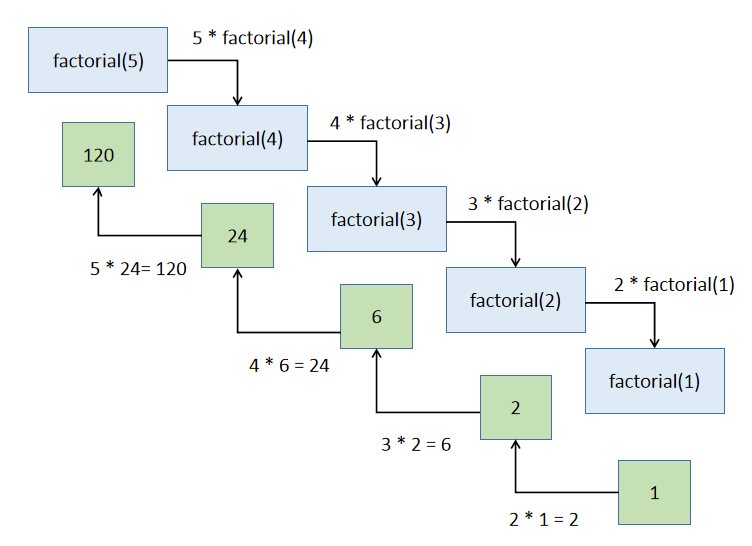
\includegraphics[]{img/C6/6-2/6.png}
% \end{figure}

% \mybox{汉诺塔}\\

% 给定三根柱子,其中A柱子从大到小套有n个圆盘,问题是如何借助B柱子,将圆盘从A搬到C。\\

% 规则:

% \begin{itemize}
% 	\item 一次只能搬动一个圆盘
% 	\item 不能将大圆盘放在小圆盘上面
% \end{itemize}

% \begin{figure}[H]
% 	\centering
% 	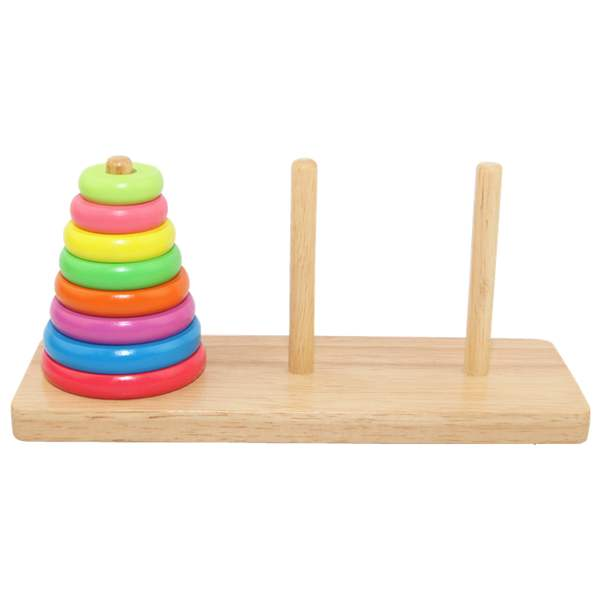
\includegraphics[scale=0.4]{img/C6/6-2/7.png}
% \end{figure}

% 递归算法求解汉诺塔问题:

% \begin{enumerate}
% 	\item 将前n-1个圆盘从A柱借助于C柱搬到B柱。
% 	\item 将最后一个圆盘直接从A柱搬到C柱。
% 	\item 将n-1个圆盘从B柱借助于A柱搬到C柱。
% \end{enumerate}

% \begin{lstlisting}[language=Python]
% public class Hanoi {
% 	public static int move = 0;		 // 移动次数

% 	public static void main(String[] args) {
% 		hanoi(4, 'A', 'B', 'C');
% 		System.out.println("步数==>" + move);
% 	}

% 	/**
% 	 * @brief  汉诺塔算法
% 	 * @note   把 n 个盘子从 src 借助 mid 移到 dst
% 	 * @param  n: 层数
% 	 * @param  src: 起点柱子
% 	 * @param  mid: 临时柱子
% 	 * @param  dst: 目标柱子
% 	 */
% 	public static void hanoi(int n, char src, char mid, char dst) {
% 		if(n == 1) {
% 			System.out.println(n + "号盘:" + src + "->" + dst);
% 			move++;
% 		} else {
% 			// 把前 n-1 个盘子从 src 借助 dst 移到 mid
% 			hanoi(n-1, src, dst, mid);
% 			// 移动第 n 个盘子
% 			System.out.println(n + "号盘:" + src + "->" + dst);
% 			move++;
% 			// 把刚才的 n-1 个盘子从 mid 借助 src 移到 dst
% 			hanoi(n-1, mid, src, dst);
% 		}
% 	}
% }
% \end{lstlisting}

% \begin{tcolorbox}
% 	\mybox{运行结果}
% 	\begin{verbatim}
% 1号盘:A -> B
% 2号盘:A -> C
% 1号盘:B -> C
% 3号盘:A -> B
% 1号盘:C -> A
% 2号盘:C -> B
% 1号盘:A -> B
% 4号盘:A -> C
% 1号盘:B -> C
% 2号盘:B -> A
% 1号盘:C -> A
% 3号盘:B -> C
% 1号盘:A -> B
% 2号盘:A -> C
% 1号盘:B -> C
% 步数 ==> 15
% \end{verbatim}
% \end{tcolorbox}

% \newpage